% Primary source: https://control.ros.org/jazzy/doc/getting_started/getting_started.html
\documentclass[tikz,border=5pt]{standalone}
\usepackage[T1]{fontenc}
\usepackage{lmodern,amsmath,amssymb}
\usetikzlibrary{arrows.meta,calc,positioning,fit,backgrounds,shapes.geometric,matrix,decorations.pathreplacing,patterns}
\definecolor{ink}{gray}{0.08}
\definecolor{wash}{gray}{0.965}
\definecolor{soft}{gray}{0.45}
\tikzset{box/.style={draw=ink,line width=.65pt,fill=white,align=center,inner sep=4pt,outer sep=0pt,font=\small},flow/.style={draw=ink,line width=.65pt,-{Latex[length=1.8mm,width=1.3mm]},rounded corners=2pt},annotation/.style={font=\scriptsize,text=soft,align=center},groupbox/.style={draw=soft,dashed,line width=.45pt,fill=wash}}
\begin{document}
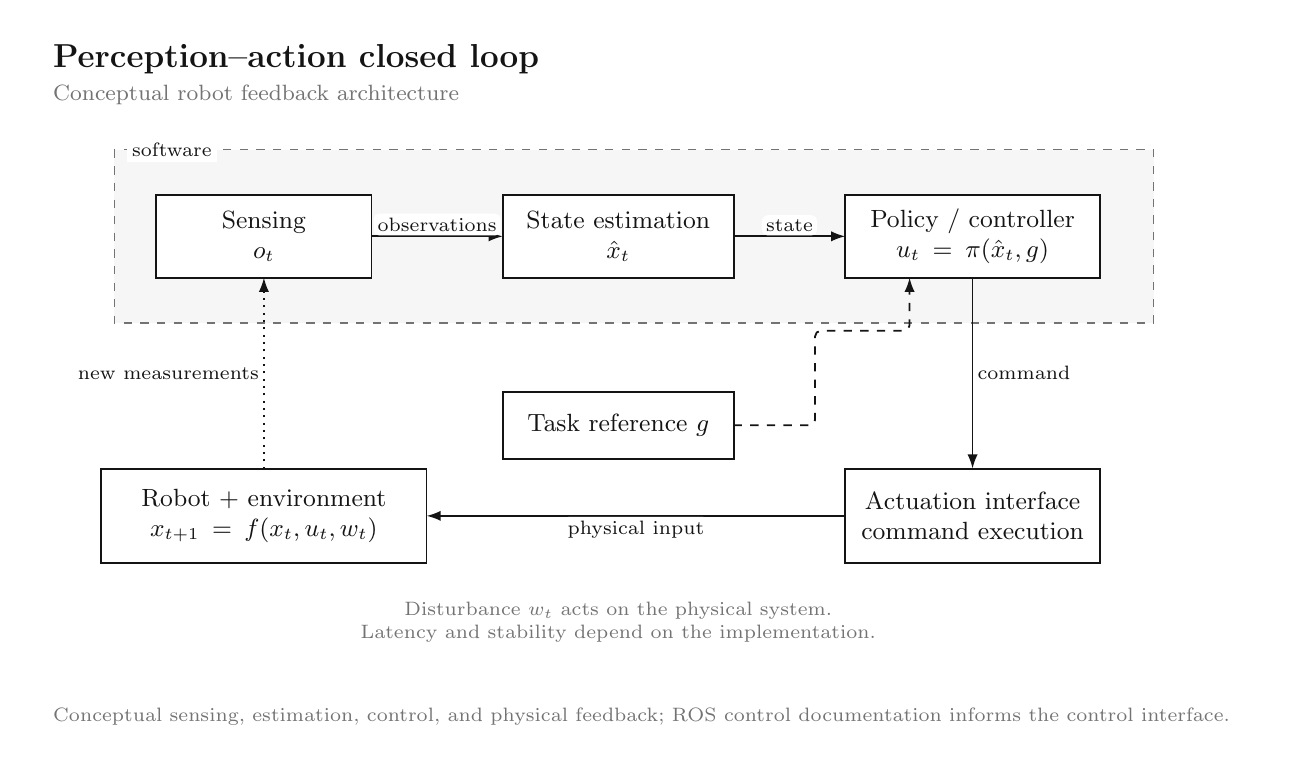
\begin{tikzpicture}[x=1cm,y=-1cm,font=\rmfamily,text=ink]

\path[use as bounding box] (0,0) rectangle (16,9);
\node[anchor=west,font=\large\bfseries] at (.2,.4) {Perception--action closed loop};
\node[anchor=west,font=\footnotesize,text=soft] at (.2,.85) {Conceptual robot feedback architecture};
\begin{pgfonlayer}{background}
\draw[groupbox] (1.1,1.55) rectangle (14.299999999999999,3.75);
\node[anchor=west,font=\scriptsize,fill=white,inner sep=2pt] at (1.25,1.55) {software};
\end{pgfonlayer}
\node[box,minimum width=2.7cm,minimum height=1.05cm,text width=2.45cm] (sense) at (3.0,2.65) {Sensing\\$o_t$};
\node[box,minimum width=2.9cm,minimum height=1.05cm,text width=2.65cm] (estimate) at (7.5,2.65) {State estimation\\$\hat{x}_t$};
\node[box,minimum width=3.2cm,minimum height=1.05cm,text width=2.95cm] (policy) at (12.0,2.65) {Policy / controller\\$u_t=\pi(\hat{x}_t,g)$};
\node[box,minimum width=4.1cm,minimum height=1.2cm,text width=3.8499999999999996cm] (world) at (3.0,6.2) {Robot + environment\\$x_{t+1}=f(x_t,u_t,w_t)$};
\node[box,minimum width=3.2cm,minimum height=1.2cm,text width=2.95cm] (actuate) at (12.0,6.2) {Actuation interface\\command execution};
\node[box,minimum width=2.9cm,minimum height=0.85cm,text width=2.65cm] (goal) at (7.5,5.05) {Task reference $g$};
\begin{pgfonlayer}{background}
\draw[flow] (sense.east) -- (estimate.west) node[midway,above,fill=white,inner sep=1.5pt,font=\scriptsize] {observations};
\draw[flow] (estimate.east) -- (policy.west) node[midway,above,fill=white,inner sep=1.5pt,font=\scriptsize] {state};
\draw[flow] (policy.south) -- (actuate.north) node[midway,right,fill=white,inner sep=1.5pt,font=\scriptsize] {command};
\draw[flow] (actuate.west) -- (world.east) node[midway,below,fill=white,inner sep=1.5pt,font=\scriptsize] {physical input};
\draw[flow,dotted] (world.north) -- (sense.south) node[midway,left,fill=white,inner sep=1.5pt,font=\scriptsize] {new measurements};
\end{pgfonlayer}
\draw[flow,dashed] (goal.east) -- (10.0,5.05) -- (10.0,3.85) -- (11.2,3.85) -- ($(policy.south)+(-.8,0)$);
\node[annotation,text width=9.3cm] at (7.5,7.55) {Disturbance $w_t$ acts on the physical system.\\Latency and stability depend on the implementation.};
\node[anchor=west,align=left,font=\scriptsize,text=soft,text width=15.6cm] at (.2,8.75) {Conceptual sensing, estimation, control, and physical feedback; ROS control documentation informs the control interface.};
\end{tikzpicture}
\end{document}
